\documentclass{article}

\usepackage{amsmath}
\usepackage[UTF8,heading=true]{ctex}
\usepackage{enumerate}
\usepackage{gensymb}
\usepackage{geometry}
\usepackage{hyperref}
\usepackage{lmodern}
\usepackage{pgfplots}
\usepackage{physics}
\usepackage{biblatex}
\usepackage{textcomp}
\usepackage{siunitx}
\usepackage{tikz}
\usepackage{ulem}

\sisetup{
      range-phrase= \sim{} ,
      range-units=single,
      list-separator=、,
      list-pair-separator=和,
      list-final-separator=和
}

\pgfplotsset{compat=1.18}

\geometry{a4paper, scale=0.8}

\numberwithin{equation}{section}
\newcommand{\gb}{《混凝土结构设计规范》(GB 50010)}
\newcommand{\gtgd}{《公路钢筋混凝土及预应力混凝土桥涵设计规范》(JTGD 62-2004)}

\newenvironment{questionList}{
      \begin{enumerate}
            \renewcommand{\labelenumi}{\chinese{enumi}、}
            \renewcommand{\labelenumii}{\arabic{enumii}.}
            \renewcommand{\labelenumiii}{(\arabic{enumiii})}
            }{
      \end{enumerate}
}

\newcommand{\subscript}[2]{
      \ensuremath{
            {#1}_{\rm{#2}}
      }
}

\pagenumbering{arabic}

\begin{document}
\title{Basic Principle of Concrete Structure}
\author{H.}
\maketitle
\newpage
\tableofcontents
\newpage
\section{绪论}
\subsection{混凝土结构的一般概念和特点}
\subsubsection{钢筋混凝土结构的一般概念}
\par 混凝土的抗拉强度一般仅为抗压强度的$1/10$左右。钢筋和混凝土结合在一起共同工作,则能各尽其用。钢筋提高了梁的承载能力、变形能力,还使梁在破坏前能给人明显的预告。
\par 施工时,一般先按构件形状尺寸制作模板,再将钢筋放入模板中适当的位置固定,最后浇筑混凝土,待混凝土结硬成型并达到一定强度时除去模板。
\subsubsection{钢筋和混凝土共同工作的原因}
\begin{itemize}
      \item 粘结性能良好;
      \item 温度线膨胀系数很接近;
      \item 混凝土包裹钢筋,可防止钢筋过早腐蚀或高温软化。
\end{itemize}
\subsubsection{预应力混凝土结构的一般概念}
\par 预压应力抵消外部荷载产生的拉应力,提高抗裂性能。
\subsubsection{混凝土结构的组成}
\par 板、梁、柱、墙和基础等。
\subsubsection{混凝土结构的优缺点}
\begin{itemize}
      \item 优点:
            \begin{itemize}
                  \item 良好的耐久性。
                  \item 良好的耐火性。
                  \item 良好的整体性。
                  \item 良好的可模性。
                  \item 可就地取材。
                  \item 节约钢材。
            \end{itemize}
      \item 缺点:
            \begin{itemize}
                  \item 自重大;
                  \item 不利于大跨、高层抗震;
                  \item 易开裂;
                  \item 现浇耗费大量模板;
                  \item 施工受季节性影响较大;
                  \item 隔热隔声性能较差等。
            \end{itemize}
\end{itemize}
\subsection{混凝土结构的发展}
\subsubsection{混凝土结构的诞生}
\subsubsection{混凝土结构材料方面的发展}
\subsubsection{混凝土结构材料体系的发展}
\subsubsection{混凝土结构的模型试验技术和计算机仿真技术}
\subsection{混凝土结构的应用}
\subsection{本课程的特点和学习方法}
\section{钢筋与混凝土材料的基本性能}
\subsection{钢筋的强度和变形}
\subsubsection{钢筋的形式和成型}
\par 混凝土结构构件中配置的钢筋可以是劲性钢筋或柔性钢筋。前者是型钢焊成的骨架。混凝土结构中更多采用柔性钢筋,柔性钢筋以下简称钢筋。
\par 钢筋按其表面形状可分为光圆钢筋和带肋钢筋(或称变形钢筋)。
\par 带肋钢筋是在钢筋表面轧制纵向肋纹(可不带)和横向斜肋纹。肋纹有螺纹、人字纹、月牙纹等多种形式。带肋钢筋截面随纵轴长度变化,直径为以重量计的当量直径。钢筋表面的肋有利于钢筋与混凝土两种材料的结合。
\begin{table}[htbp]
      \caption{钢筋的直径(单位为$mm$)}
      \begin{center}
            \begin{tabular}{|c|ccccccccc|cccccc|}
                  \hline
                  光圆钢筋 & 6 & 8 & 10 & 12 & 14 & 16 & 18 & 20 & 22 &    &    &    &    &    &    \\
                  \hline
                  带肋钢筋 & 6 & 8 & 10 & 12 & 14 & 16 & 18 & 20 & 22 & 25 & 28 & 32 & 36 & 40 & 50 \\
                  \hline
            \end{tabular}
      \end{center}
\end{table}
\par 直径较小的钢筋也称钢丝,通常为光圆外形,若在表面机械刻痕以提高粘结力,则称刻痕钢丝。多股钢丝捻在一起形成的钢绞线也可以作为配筋。
\par 浇筑前可以将布置在构件中的各种钢筋用绑扎或焊接的方法做成钢筋骨架或钢筋网片,就可以保持其相对位置,有利于发挥钢筋的强度。
\begin{itemize}
      \item 为了防止受拉的光面钢筋滑动,应在其端部设弯钩。
      \item 为了设计的要求\footnote{比如受拉、受压侧的互换等。},有时还需在钢筋中间区段弯转。
      \item 受压的光面钢筋端部可不设弯钩,因为钢筋受压时周围的混凝土会约束其截面膨胀或偏移,进而有利于阻止其滑动。
      \item 带肋钢筋表面有齿肋花纹,与混凝土有很好的结合性能,端部可不设弯钩。有时为了满足锚固长度的要求而必须设置时,采用较易成形的直角型弯钩。
      \item 焊接方法制成的钢筋骨架或钢筋网片,能与混凝土较好地结合,钢筋端部可不设置弯钩。
\end{itemize}
\par 为了保证钢筋在加工、使用时不开裂、弯断和脆断,通常用冷弯试验\footnote{用外力使钢筋围绕一定直径的辊轴弯转,在达到规定的弯转角度后钢筋不能出现裂纹或断裂。}来检验其韧性和内部质量。焊接的钢筋骨架和网片省工省料、适用于工业化批量生产、装配式结构的生产,能减少工作量,加快施工进度。需要焊接的钢筋应具有较好的可焊性。
\subsubsection{单调荷载下钢筋的强度和变形}
\par 常规的荷载试验通常采用单调加载。
\par 热轧低碳钢和普通热轧低合金钢等应力--应变关系随应变增加表现为:线性--比例极限--轻微非线性--流幅(屈服台阶)--强化--极限点--颈缩--断裂。
\par 高碳钢应力--应变关系中没有明显的屈服点和流幅,一般取残余应变为$0.2\%$时对应的应力$\sigma_{0.2}$作为钢筋的条件屈服强度。但冶金系统产品标准中规定屈服强度$\sigma_{0.2}$不得小于极限抗拉强度$\sigma_b$的$85\%$,因此实际应用中可取极限抗拉强度$\sigma_b$的$85\%$作为条件屈服点。
\par 具有明显流幅的钢材统称为软钢,无明显流幅的钢材统称为硬钢。流幅$\varepsilon_{sh}$和极限应变$\varepsilon_{su}$是较重要的塑性指标。软钢的应力--应变关系通常采用理想弹塑性模型(两折线模型),即
$$
      \sigma_s =
      \left\{ \begin{aligned}
            E_s \varepsilon_s & (\varepsilon_s \leq \varepsilon_y) \\
            f_y               & (\varepsilon_s >\varepsilon_y)
      \end{aligned} \right.
$$
\par 钢筋可根据化学成分分为碳素钢、普通合金钢两大类,根据加工方式分为热轧钢筋、冷拉钢筋和热处理钢筋三大类。
\par 钢筋强度标准值取强度平均值减去两倍标准差时,保证率可达到97.73\%。\gb{}采用概率极限状态设计法,于是钢筋强度设计值等于钢筋强度标准值除以钢筋材料分项系数$\gamma_s=1.1$;还规定,对结构构件进行承载力设计时,采用钢筋强度设计值,进行变形和裂缝宽度验算时,采用钢筋强度标准值。
\subsubsection{钢筋的冷加工和热处理}
\par 冷拉或冷拔的冷加工方法可以提高热轧钢筋的强度。
\par 冷拉加工是在常温下把软钢拉伸到超过屈服强度的某一应力值,然后卸去拉力。此时将产生残余应变,不再有明显的屈服台阶,塑性变差,抗拉强度提高,抗压强度不变。
\par 如果卸去拉力后在自然条件下放置一段时间后再进行拉伸,则屈服点可进一步提高,这种现象称为时效硬化。原材料强度越高,冷拉加工提高幅度越小。温度达\SI{70}{\degreeCelsius}时,冷拉的效果消失,因此需要焊接和冷拉的钢筋应先焊接再冷拉。
\par 冷拔加工是用强力将钢筋拔过硬质合金拔丝模上比其直径稍小的锥形孔,这时钢筋会在轴向拉力和横向挤压力的同时作用下产生塑性变形,横截面减小,长度增加,内部结构发生变化,抗拉抗压强度同时提高。多次冷拔后,钢筋的塑性明显降低,没有明显的屈服点和流幅。
\subsubsection{钢筋的徐变和松弛}
\par 钢筋在较高应力的持续作用下,应变会随时间增长继续增加,这种现象称为徐变;若保持受力钢筋长度不变,则应力会随时间增长降低,这种现象称为松弛。
\par 通常,初始应力大,徐变或松弛损失也大;冷拉热轧钢筋的徐变或松弛较冷拔低碳钢丝、碳素钢丝和钢绞线更低;温度增加,徐变或松弛也增大。
\subsubsection{重复和反复荷载下钢筋的强度和变形}
\par 重复荷载指同一方向反复加载卸载。应力--应变关系曲线的包络图与单调荷载下的应力--应变关系曲线几乎相同。
\par 反复荷载指在相反方向交替加载卸载。若加载超过屈服应变后卸载,应力--应变关系曲线沿加载直线平行方向下行,再反向加载时,立即塑性变形,弹性极限相对单调荷载下降低,这种现象称为“包兴格效应”。
\par 钢筋承受周期性的重复荷载后,可能在未达到单调加载时的强度时破坏,这种现象称为疲劳破坏。疲劳强度指在规定应力范围内,经受一定次数循环荷载后发生疲劳破坏的最大应力值;它与应力幅限值(一次循环应力中最大与最小应力间的差值)、钢筋表面的形状、钢筋的直径、强度、加工使用的环境和加载的频率等有关。疲劳应力比值是指同一层钢筋的最小应力与最大应力的比值。
\subsection{混凝土的强度和变形}
\par 普通混凝土是由水泥、砂、石材料用水拌合硬化后形成的人工石材,一种复杂的多相复合材料。其中的砂、石、水泥胶块中的晶体、未水化的水泥颗粒组成了弹性骨架,水泥胶块中的凝胶、孔隙和结合界面的初始微裂缝则为塑性变形提供可能。孔隙、初始裂缝等先天缺陷往往是混凝土受力破坏的起因,而且微裂缝的开展对力学性能有极为重要的影响。
\subsubsection{混凝土立方体受压}
\par 混凝土立方体抗压强度是确定混凝土强度等级的依据,\gb{}规定混凝土强度按立方体抗压强度标准值$f_{cu,k}$确定。
\par 混凝土强度与水泥强度等级、水灰比关系很大,也受骨料的性质、混凝土的级配、混凝土成形方法、硬化时的环境条件及混凝土的龄期等影响;试验时试件的大小形状、试验方法和加载速率也会影响测得的强度;加载速度下降,峰值应力也略有降低,相应的应变有所增加,下降段的坡度趋于平缓。
\subsubsection{混凝土轴心受压}
\par 混凝土棱柱体试件试验得到的轴心抗拉强度值能更好地反映混凝土结构构件中混凝土实际抗压能力。混凝土轴心抗压强度设计值$f_c$是轴心抗压强度标准值$f_{ck}$除以混凝土材料分项系数$\gamma_c=1.4$得到的。而\gb{}偏于安全地使用
$$
      f_{ck} = 0.88 \alpha_1 \alpha_2 f_{cu,k}
$$
\par 其中,$\alpha_1$为棱柱体强度与立方体强度之比,$\alpha_2$为高强度混凝土的脆性折减系数。0.88是考虑到实际结构构件制作、养护和受力情况以及实际构件与试件混凝土强度之间的差异而取用的折减系数。
\begin{center}
      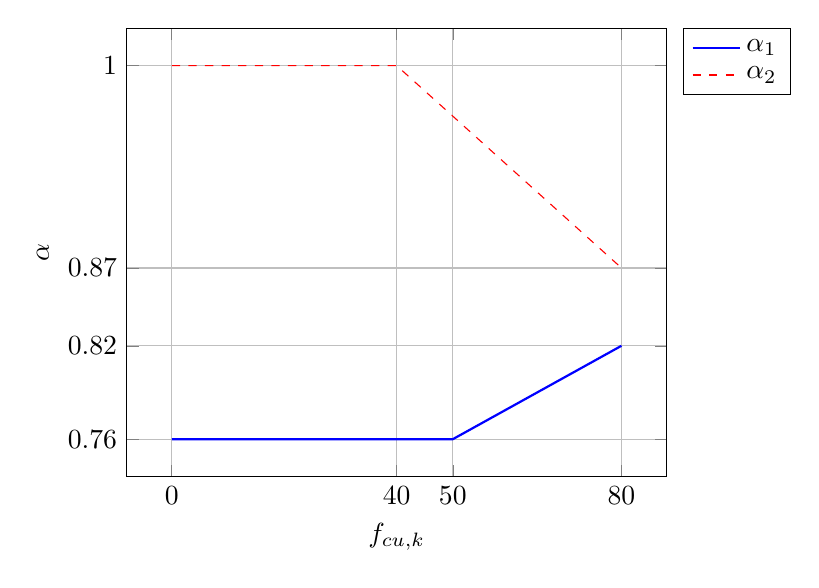
\begin{tikzpicture}
            \begin{axis}[
                        xlabel={$f_{cu,k}$},
                        ylabel={$\alpha$},
                        samples=200,
                        grid,
                        domain=0:80,
                        legend pos=outer north east,
                        smooth,
                        xtick={0,40,50,80},
                        ytick={0.76,0.82,0.87,1.00},
                  ]
                  \addplot [no marks, sharp plot, blue, thick] coordinates{(0,0.76) (50,0.76) (80,0.82)};
                  \addlegendentry{$\alpha_1$}
                  \addplot [no marks, sharp plot, red, dashed] coordinates{(0,1.00) (40,1.00) (80,0.87)};
                  \addlegendentry{$\alpha_2$}
            \end{axis}
      \end{tikzpicture}
\end{center}
\par 强度等级不同的混凝土,应力--应变关系曲线形状相似,但也有实质性的差别。混凝土的强度越高,下降段的坡度就越陡,变形性能也就越差。
\par \gb{}结合近年对高强混凝土的研究成果提出的混凝土轴心受压时的应力--应变关系的数学表达式为\footnote{显然$\Delta f_{cu}$是我新定义的。}
\begin{align*}
      \sigma_c         & =
      \left\{ \begin{aligned}
                     & f_c[1-(1-\frac{\varepsilon_c}{\varepsilon_0})^n] & \varepsilon_c \leq \varepsilon_0                    \\
                     & f_c                                              & \varepsilon_0 < \varepsilon_c \leq \varepsilon_{cu}
              \end{aligned} \right. \\
      \Delta f_{cu}    & = \max \{f_{cu}-50, 0\}                                                                        \\
      n                & = 2 - \frac{1}{60} \Delta f_{cu}                                                               \\
      \varepsilon_0    & =0.002 + 0.5 \Delta f_{cu} \times 10^{-5}                                                      \\
      \varepsilon_{cu} & =0.0033 - \Delta f_{cu} \times 10^{-5}
\end{align*}
\par 当$f_{cu} \leq 50\rm{MP_a}$时,上式变为
\begin{align*}
      \sigma_c         & =
      \left\{ \begin{aligned}
                     & f_c[1-(1-\frac{\varepsilon_c}{\varepsilon_0})^2] & \varepsilon_c \leq \varepsilon_0                    \\
                     & f_c                                              & \varepsilon_0 < \varepsilon_c \leq \varepsilon_{cu}
              \end{aligned} \right. \\
      \varepsilon_0    & =0.002                                                                                         \\
      \varepsilon_{cu} & =0.0033
\end{align*}
\par 混凝土受压时,泊松比由弹性阶段($\sigma_c<0.5f_c$)的$1/6$逐渐增加到接近破坏时的$0.5$以上。
\subsubsection{混凝土受拉}
\par 混凝土轴心抗拉试验的标准试件是两端预埋钢筋的棱柱体,也常用圆柱体或立方体的劈裂试验\footnote{劈裂截面上除了受压点附近外均为受拉状态。}来间接测试混凝土的抗拉强度,一般劈裂抗拉强度仅略高于直接受拉强度。
\par 根据试验资料,混凝土轴心抗拉强度与立方体抗压强度的关系是
$$
      f_t = 0.395 f_{cu}^{0.55}
$$
\par \gb{}给出混凝土轴心抗拉强度的标准值与立方体抗压强度标准值的关系是
$$
      f_tk = 0.88 \times 0.395 f_{cu,k}^{0.55} (1-1.645\delta)^{0.45}\times \alpha_2
$$
\par 混凝土轴心受拉应力--应变关系曲线的形状与受压应力--应变关系曲线相似,但下降段较陡;下降段随混凝土强度提高变得更加陡峭。混凝土轴心受拉应力--应变关系曲线一般用双直线模型模拟,且认为混凝土受拉弹性模量与受压弹性模量相等。
\subsubsection{复合应力状态下混凝土强度}
\par 双向压拉受拉强度$<$双向受拉强度$\approx$单轴受拉强度$<$双向压拉受压强度$<$单轴受压强度$<$双向受压强度。
\par 在$0.5f_c$范围内,抗剪强度随压应力增大而提高,接下来抗剪强度则随压应力增大而降低,但直到$09f_c$以上才降低到原先的抗剪强度;抗剪强度随着拉应力增大而降低。剪应力会降低抗压强度和抗拉强度。
\par 合适的侧向约束压力可以提高轴向抗压强度和可塑性,所以可以配置圆箍筋或螺旋箍筋来提高受压承载力和变形性能。
\subsubsection{重复荷载下混凝土的强度和变形}
\par 加载到$\varepsilon_c$并卸载后,相当一部分应变$\varepsilon_e^{\prime}$可以瞬时恢复,隔一段时间后还能再恢复一部分应变$\varepsilon_c^{\prime}$,称为弹性后效,剩下的部分应变$\varepsilon_{cr}^{\prime}$不能恢复,称为残余应变。
\par 重复荷载加载应力小于混凝土疲劳强度时,加载和卸载过程形成的环状曲线趋于闭合,不会破坏;反之,加载阶段应力--应变关系曲线由凸向应力轴逐渐变成直线,再逐渐凸向应变轴,以致不能形成封闭的环形,最终发生疲劳破坏。
\subsubsection{长期荷载下混凝土的变形}
\par 应力保持不变的条件下,混凝土的应变会随时间持续而增大,这种现象称为徐变。加载的前几个月徐变增长较快,此后增长速度逐渐减慢。卸载后徐变也分为瞬时恢复应变、弹性后效和残余应变三部分。
\par 徐变会加大构件的变形、引起截面应力重分布、引起预应力损失。
\par 应力大小是徐变的重要因素,$\sigma_c\leq0.5f_c$时基本呈正比,称为线性徐变。
\par 混凝土的水灰比越大,徐变越大;水泥用量越多,徐变也越大;采用坚硬的、弹性模量大的骨料有利于减小徐变;增加混凝土中骨料所占体积比也有利于减小徐变。
\par 在温度和湿度较高的条件下养护能促进水化作用,减小徐变;如果受载期间所处环境的温度较高而湿度较低则会增大徐变;加载龄期越短徐变越大。
\par 形状和尺寸会影响徐变值,尺寸较大时水分不易丢失,徐变较小。
\subsubsection{混凝土的收缩、膨胀和温度变形}
\par 混凝土在空气中凝结硬化时会收缩,在水中凝结硬化时会膨胀。
\begin{itemize}
      \item 水泥等级越高,收缩越大。
      \item 水泥用量越多,收缩越大;水灰比越大,收缩也越大。
      \item 骨料的弹性模量越大,收缩越小。
      \item 结硬和使用过程中,周围湿度越大,收缩越小。湿度大时,养护温度越高,收缩越小;湿度小时,养护温度越高,收缩越大。\footnote{温度升高只是促进水分的输运。}
      \item 混凝土振捣得越密实,收缩越小。
      \item 构件的体积与表面积的比值越大,收缩越小。
\end{itemize}
\par 混凝土构件养护不好或自由收缩受到约束时会出现裂缝。
\par 混凝土硬化的膨胀值比收缩值小得多,且对受力有利,所以不考虑膨胀。
\par 混凝土的线膨胀系数与配合比和骨料性质有关。温度变化在钢筋与混凝土之间引起的变形相差很小,不会产生有害的内应力。但大体积混凝土结构\footnote{温度不均匀。}以及水池、烟囱\footnote{温度变化相对频繁。}等结构应考虑温度应力的影响。
\section{粘结与锚固}
\subsection{粘结作用与粘结机理}
\subsubsection{裂缝出现前的粘结作用}
\par 钢筋和混凝土之间的粘结应力是由于变形差(相对滑移)沿钢筋与混凝土接触面上产生的剪应力,它们能够共同工作的基本前提就是能够承受粘结应力的粘结强度。
\par 出现裂缝前,由于梁的剪弯段中钢筋的拉应力不恒定,所以钢筋和混凝土之间有粘结作用,而且其分布规律还会受微裂缝的影响、
\subsubsection{裂缝出现后的粘结作用}
\par 裂缝出现后。钢筋和混凝土之间的粘结作用分为锚固粘结和裂缝间的局部粘结。
\par 为了避免钢筋在拉力作用下被拔出,梁内锚固部位(一般是支座、两端)的钢筋被混凝土紧紧“握住”,这种粘结作用称为锚固粘结,它是通过混凝土和钢筋之间一定长度粘结应力的累积实现的。
\par 钢筋需要在构件中间切断、长度不够或者需要设置施工缝时,在接头处需要延伸或者搭接。锚固不足时构件将提前破坏。
\par 裂缝出现前的粘结作用也属于锚固粘结。
\par 裂缝处拉力全部由钢筋承担,但裂缝间钢筋的拉力可以通过粘结应力部分地向混凝土传递,使未开裂的混凝土受拉,这种粘结应力称为裂缝间粘结应力,它能改善钢筋混凝土梁的耗能性能\footnote{?}。
\subsubsection{粘结试验}
\par 最早的粘结试验\footnote{粘结试验是指研究钢筋与混凝土间粘结性能的试验。}装置是拔出试验。它是将钢筋沿纵轴对称劈开后在内放置应变片后合拢并用环氧树脂粘牢,用该钢筋浇筑拔出试件,置于有孔的支座上,通过孔在钢筋上施加逐步加大的向下拉力,直至拔出。可用应变推出应力,于是记钢筋截面积为$A_s$,周长为$\mu_s$,则粘结应力
$$\tau=\derivative{\sigma_s}{x}\frac{A_s}{\mu_s}$$
\par 试验得到的结果主要有
\begin{enumerate}
      \item 对拔出前某一受拉状态,只有靠近端部的部分钢筋能达到最大钢筋应力,也主要在一部分长度内产生粘结应力。这段长度称为应力传递长度,或简称传递长度。
      \item 传递长度范围内不同位置处钢筋与混凝土之间的粘结应力的大小不同,拔出试验难以测得粘结强度。
\end{enumerate}
\par 针对实际构件中混凝土的受力状态不同于试件状态\footnote{比如拔出试验中,钢筋向下拔出,混凝土立置于支座上受压,会导致构件横向膨胀。},也有很多对该实验的改进。而与受拉状态下的拔出试验对应的,也可进行受压状态下的挤压试验。
\subsubsection{粘结机理及粘结破坏形态}
\par 光圆钢筋的粘结作用由三部分组成:
\begin{enumerate}
      \item 混凝土中水泥胶体与钢筋表面的\underline{化学胶着力};
      \item 钢筋与混凝土接触面上的\underline{摩擦力};
      \item 钢筋表面粗糙不平产生的\underline{机械咬合力}\footnote{尤其是微锈情况下。}。
\end{enumerate}
\par 其中胶合力所占比例很小,相对滑移后,粘结力主要由摩擦力和机械咬合力提供。
\par 带肋钢筋的粘结作用中,前两部分基本相同,而第三部分主要表现为钢筋表面突出的\underline{肋}与混凝土的机械咬合作用。
\par 肋对混凝土斜向挤压力的径向分量对不同侧的混凝土分别有压拉作用,轴向分量则使肋间混凝土受剪弯作用;因此带肋钢筋的外围混凝土处于极其复杂的三向应力状态,当径向分量足够大时,就会产生劈裂裂缝,发生局部挤碎,或者因钢筋被拔出而受到刮出式破坏。
\par 钢筋受压时钢筋和端部混凝土的局部挤压和泊松效应导致的钢筋直径变大则会明显延缓粘结破坏。
\subsubsection{搭接的工作机理}
\par 搭接区一端的钢筋通过与混凝土之间的粘结将其所受的力传给另一端的钢筋。
\subsection{钢筋与混凝土之间的粘结强度}
\subsubsection{粘结强度}
\par 拔出试验中,如果钢筋埋入长度足够短,就可以近似认为粘结应力沿钢筋纵轴方向均匀分布,可以在一部分长度上加设套管,保证部分区域内钢筋与混凝土之间无粘结,来测试钢筋与混凝土之间的粘结强度。记测得的拔出拉力为$T_u$,钢筋的埋置长度为$l_c$,则
$$\tau_u=\frac{T_u}{\mu_sl_c}$$
\subsubsection{影响粘结强度的因素}
\par 粘结强度随\underline{混凝土强度}等级的提高而提高,且与劈裂抗拉强度近似成正比。
\par \underline{浇筑深度}超过300mm的“顶部”水平钢筋,由于钢筋底面的混凝土水分析出、气泡逸出和混凝土泌水下沉等而不能与钢筋紧密接触,粘结作用削弱,要比竖位钢筋和“底部”钢筋低20\%\texttildelow30\%。
\par 带肋钢筋具有比光圆钢筋更高的粘结强度,但主要危险是产生劈裂裂缝而非发生滑移。增大混凝土\underline{保护层厚度}和保持一定的钢筋净距,可以提高外围混凝土的劈裂抗力,保证粘结强度。
\par 横向钢筋能延缓内裂缝的发展,提高粘结强度、限制到达构件表面的劈裂裂缝的宽度。因此搭接区和较大直径钢筋的锚固区内,均应设置一定数量的横向钢筋(如环状箍筋);当一排并列钢筋的根数较多时,还应设置附加钢箍以防止保护层混凝土的劈裂剥落。
\par 当钢筋的锚固区作用有横向压应力时,其能制约混凝土的横向变形,增大摩阻力,可以抵抗滑动,进而提高粘结强度。因此在直接支承的支座处可以适当减小锚固长度。
\par 带肋钢筋的外形特征对粘结强度有不显著的影响。
\subsection{钢筋在混凝土中的锚固长度}
\subsubsection{锚固长度的理论分析}
\par 保证锚固可靠就是要求钢筋屈服时锚固仍未破坏,通常需要将钢筋在混凝土中延伸一段长度,即锚固长度。确定锚固长度的基本原则是钢筋受力屈服时正好发生锚固破坏。
\par 拔出试验是确定钢筋锚固长度最直接的办法。根据
\subsection{实用的锚固长度计算公式}
\par 下式中$\alpha$的值大约是$1/6$。
$$l_a=\alpha \frac{f_y}{f_t}d$$
\section{轴心受力构件的性能与计算}
\subsection{工程实例及构件的配筋形式}
\par 纵向钢筋的目的是\begin{enumerate}
      \item 协助混凝土承受压力以减小构件截面尺寸;
      \item 承受可能有的不大的弯矩;
      \item 防止构件突然脆性破坏。
\end{enumerate}
\subsection{轴心受拉构件的受力分析}
\subsubsection{轴力受拉构件试验研究}
\par 开裂前、开裂后、屈服三个阶段。
\par 裂缝处的混凝土不再承受拉力。
\subsubsection{轴向拉力与变形的关系}
\par 弹性模量比$\alpha_E=E_s/E_c$
\par 构件截面积。
\par 等效截面积$A_0=(1+\alpha_E\rho)$
\par 开裂荷载$N_{tcr}=E_cA(1+\alpha_E\rho)\epsilon_{t0}$
\par 极限荷载$N_{tu}=f_yA_s$
\subsection{轴心受拉构件承载力计算公式的应用}
\subsubsection{既有构件轴心抗拉承载力计算}
\par 取开裂荷载和极限荷载的最大值。
\subsubsection{基于承载力的构件截面设计}
$\rho_{min} = \frac{A_{smin}}{A} \approx \frac{f_t}{f_y}$
\subsection{轴心受压短柱的受力分析}
\subsubsection{短柱的试验研究}
\par 屈服前、屈服后直至开裂两个阶段。
\subsubsection{短柱压力与变形的关系}
\par 混凝土压力与变形的关系$N_c^c=1000\epsilon(1-250\epsilon)f_cA$
\subsubsection{荷载长期作用下短柱的受力性能}
\par 徐变系数$C_t=\frac{\varepsilon_{cr}}{\varepsilon_i}$
\subsection{轴心受压长柱的受力分析}
\subsubsection{长柱的试验研究}
\subsubsection{稳定系数}
\subsubsection{轴心受压柱的承载力计算公式}
\par $N_{cu}=\varphi f_cA+f_y^{\prime}A_s^{\prime}$
\subsection{轴心受压构件承载力计算公式的应用}
\subsubsection{既有构件轴心抗压承载力计算}
\subsubsection{基于承载力的构件截面设计}
\subsection{配有纵筋和螺旋筋轴心受压柱的受力分析}
\subsubsection{螺旋筋柱的轴心受压试验研究}
\subsubsection{螺旋筋柱的承载力计算}
\par $f_{cc}=f_c+4\alpha\sigma_r$
\par 由$2f_yA_{ss1}=\sigma_rsd_{cor}$,$\sigma_r=\frac{2f_yA_{ss1}}{sd_{cor}}=\frac{f_yA_{ss0}}{2A_{cor}}$
\par $N_{cu}=f_{cc}A_{cor}+f_y^{\prime}A_s^{\prime}=f_cA_{cor}+f_y^{\prime}A_s^{\prime}+2f_yA_{ss0}$
\section{受弯构件正截面的性能与计算}
\subsection{工程应用实例}
\par 受弯构件截面可以有多种形状,但由于受压翼缘(可能有折减)和腹板可分别合并到中间,可归纳为矩形截面和T形截面\footnote{当然合并到到中间后也不一定为T形,但是这样的截面通常对受力并没有太大帮助。},其差别在于受压部分是否增加宽度。
\subsection{受弯构件的受力特点和配筋形式}
\par 钢筋混凝土梁中通常配有用于受弯的纵筋、用于受剪的弯筋与箍筋和用于架立前述钢筋的架立筋。钢筋混凝土板中通常仅配有纵筋和用于固定的分布钢筋。
\subsection{受弯构件的截面尺寸和配筋构造}
\par 梁的宽度$b$(\unit{\mm})通常取
$$
      150, 180, 200, 220, 250...50...\infty
$$
梁的高度$h$(\unit{\mm})通常取
$$
      200...50...800,800...100...\infty
$$
箍筋的直径\unit{\mm}通常取
$$
      6...2...12
$$
\par 对于钢筋混凝土受弯构件,受压区钢筋净距不小于$\max(30mm, d_s^{\prime})$,受拉区钢筋净距(横向和纵向)不小于$\max(25mm, d_s)$,保护层厚度$c \ge \max(25mm, d_s)$。
\subsection{受弯构件正截面性能的试验研究}
\par 弯矩-曲率关系曲线和荷载-位移关系曲线。
\subsection{单筋矩形截面受弯构件正截面的受力分析}
\subsubsection{受压区混凝土等效矩形应力图形}
\par 将宽$b$高$x_n$且应力不均匀的混凝土受压区简化为宽$b$高$x$且应力均匀的混凝土受压区。简化时的假设为受压区顶端位置保持不变,底端位置上移,受压区合力位置、大小不变。
\par 简化前的受压区最大应力显然为$f_c$,简化后的受压区应力为$\alpha_1f_c$;简化前的受压区高度为$x_n$,简化后的受压区高度为$x=\beta_1x_n$。
\subsubsection{界限受压区高度}
\par 假设混凝土压碎时钢筋恰屈服,由几何关系有
\begin{align}
      \frac{x_n}{h_0-x_n} & = \frac{\varepsilon_{cu}}{\varepsilon_y}                  \\
      \frac{x_n}{h_0}     & = \frac{\varepsilon_{cu}}{\varepsilon_{cu}+\varepsilon_y} \\
                          & = \frac{1}{1+\frac{\varepsilon_y}{\varepsilon_{cu}}}      \\
                          & = \frac{1}{1+\frac{f_y}{E_s\varepsilon_{cu}}}
\end{align}
记此时的$x_n$为$x_{nb}$,$x$为$x_b$,则
\begin{align}
      x_b = \beta_1x_{nb}=\frac{\beta_1}{1+\frac{f_y}{E_s\varepsilon_{cu}}}
\end{align}
\subsubsection{极限承载力高度}
\par 受压区合力作用点与受拉钢筋合力作用点的距离为$h_0-x/2$
\subsection{单筋矩形截面受弯构件正截面承载力的简化分析}
\subsection{单筋矩形截面受弯构件正截面承载力计算公式的应用}
\subsection{双筋矩形截面受弯构件正截面承载力的受力分析}
\subsection{双筋矩形截面受弯构件正截面承载力计算公式的应用}
\appendix
\newpage
%\newcommand{\ans}{\setlength{\par indent}{-2em}\par 答:\setlength{\par indent}{0em}}
\newcommand{\ans}{\par \noindent \textbf{答:}}
%\newcommand{\ans}{\par 答:}
\section{思考题}
\begin{enumerate}
      \item
            \begin{enumerate}[1.]
                  \item 钢筋和混凝土共同工作的基础是什么?
                        \ans 有三点,两者之间良好的粘结性能、相近的温度线膨胀系数、混凝土对钢筋的包裹带来的对钢筋锈蚀或高温软化的抑制作用。
                  \item 与素混凝土相比,钢筋混凝土梁有哪些优势?
                        \ans 提高梁的承载能力、变形能力,并使其在破坏前能预警。
                  \item 与钢筋混凝土梁相比,预应力混凝土梁有哪些优势?
                        \ans 预应力产生的预压应力会抵消(全部或大部分)外部荷载产生的拉应力,提高抗裂性能。
                  \item 与其他结构相比,混凝土结构有哪些特点?
                        \ans 优点有:良好的耐久性、耐火性、整体性、可模性,可就地取材,节约钢材。缺点有:自重大,对大跨、高层抗震不利,易开裂,现浇需耗费大量模板,施工受季节性影响较大,隔热隔声性能较差等。
            \end{enumerate}
      \item \begin{enumerate}[1.]
                  \item 钢筋可以如何分类?
                        \ans 钢筋按其表面形状可分为光圆钢筋和带肋钢筋,根据化学成分可分为碳素钢、普通合金钢两大类,根据加工方式可分为热轧钢筋、冷拉钢筋和热处理钢筋三大类。
                  \item 软钢和硬钢的应力--应变关系曲线有何不同?它们的屈服强度是如何取值的?
                        \ans 不同在前者有明显的屈服平台和流幅,而后者没有。软钢的屈服强度为屈服点(其实屈服点还可以细分)对应的强度,硬钢的屈服强度为条件屈服点(残余应变为$2\%$或极限抗拉强度的$85\%$)对应的强度。
                  \item 钢筋应力--应变关系曲线的理论模型有哪几种?它们适用于何种情况?
                        \ans 三折线模型适用于软钢,两折线模型适用于流幅较长的钢筋和实际应用中的普通钢筋,双斜线模型适用于无明显流幅的高强钢筋或钢丝。
                  \item 冷拉和冷拔会对钢筋的力学性能有怎样的影响?
                        \ans 冷拉后不再有明显的屈服台阶,塑性变差,抗拉强度提高,抗压强度不变;冷拉后静置一段时间再进行冷拉,可进一步提高屈服点。多次冷拔后,钢筋的塑性明显降低,没有明显的屈服点和流幅。
                  \item 对混凝土结构中的钢筋性能有哪些要求?
                        \ans 冷弯性能、需要焊接时的可焊性。
                  \item 如何确定混凝土立方体抗压强度、轴心抗压强度和轴心抗拉强度?
                        \ans 分别通过混凝土立方体抗压试验、混凝土棱柱体抗压试验和轴心抗拉试验(或劈裂抗拉试验)。
                  \item 混凝土强度等级是如何确定的?\gb{}覆盖的混凝土强度等级范围是什么?
                        \ans 依据混凝土立方体抗压强度标准值。C15到C80。
                  \item 混凝土轴心受压应力--应变关系曲线的主要特点是什么?试举一常用的应力--应变关系数学模型加以说明。
                        \ans 分为上升段和下降段,上升段应力上升速率逐渐放缓,由原先接近直线的状态变为上凸。比如E. Hognestad建议的模型中,上升段取为二次抛物线,下降段取为斜直线。
                  \item 如何确定混凝土的变形模量和弹性模量?
                        \ans 变形模量有三种表示方法,包括通常所指的弹性模量---原点弹性模量,从应力--应变关系曲线上求得。
                  \item 什么是混凝土的疲劳强度?重复荷载下混凝土应力--应变关系曲线有何特点?
                        \ans 多次重复荷载作用下能够保证构件不疲劳破坏的最大加载应力。加载应力小于疲劳强度时趋于闭合,反之无法闭合,应变持续增大,最终疲劳破坏。
                  \item 什么是混凝土的徐变和收缩?影响混凝土徐变和收缩的因素有哪些?
                        \ans 徐变是指应力保持不变的情况下,混凝土的应变随时间推移而增大。影响混凝土徐变的因素有应力大小、内在因素(组成成分、形状尺寸)、环境影响(制作方法、龄期和以温湿度为主的养护条件)等。
                        \par 收缩是混凝土在空气中凝结硬化时体积缩小的现象。影响混凝土收缩的因素有:水泥品种、水泥用量、骨料性质、外部环境、施工质量和构件体表比等。
                  \item 混凝土的徐变和收缩对钢筋混凝土构件的受力状态各有何影响?
                        \ans 徐变会加大构件的变形、引起钢筋混凝土截面(或其他组合截面)应力重分布、引起预应力损失。收缩可能造成裂缝,影响观瞻且不利于构件使用性能和耐久性能。
            \end{enumerate}
      \item  \begin{enumerate}[1.]
                  \item 什么是钢筋与混凝土之间的粘结作用?有哪些类型?
                        \ans 粘结作用是指钢筋和混凝土之间通过接触面上剪应力避免变形差从而共同工作的作用。
                  \item 钢筋与混凝土间的粘结力有哪几部分组成?哪一种作用为主要作用?
                        \ans  光圆钢筋与混凝土的粘结作用由三部分组成:\begin{enumerate}
                              \item 混凝土中水泥胶体与钢筋表面的化学胶着力;
                              \item 钢筋与混凝土接触面上的摩擦力;(主要)
                              \item 钢筋表面粗糙不平产生的机械咬合作用。(主要)
                        \end{enumerate}
                        \par 带肋钢筋与混凝土的粘结作用也由三部分组成:\begin{enumerate}
                              \item 混凝土中水泥胶体与钢筋表面的化学胶着力;
                              \item 钢筋与混凝土接触面上的摩擦力;
                              \item 钢筋表面凸出的肋与混凝土的机械咬合作用。(主要)
                        \end{enumerate}
                  \item 带肋钢筋的粘结破坏形态有哪些?
                        \ans  径向分量引起梁底或梁侧的纵向裂缝,纵向分量引起的混凝土撕裂、局部挤碎或刮出式破坏。
                  \item 影响钢筋与混凝土之间的粘结强度的主要因素有哪些?
                        \ans  混凝土强度、浇注位置、保护层厚度、钢筋净距离、横向配筋及侧向压应力等。
                  \item 确定基本锚固长度的原则是什么?如何确定钢筋的基本锚固长度?
                        \ans  原则是要求钢筋屈服时仍未出现锚固破坏。确定钢筋的基本锚固长度最直接的方法是拔出试验。
                  \item 对水平浇筑的钢筋混凝土梁,其顶部钢筋与混凝土间的粘结强度和底部钢筋与混凝土间的粘结强度相比有何区别?为什么?
                        \ans 顶部混凝土由于水分、气泡的逸出和混凝土泌水下沉,相对较疏松,削弱了粘结作用。
                  \item 两根钢筋在混凝土中搭接时是否允许钢筋并拢?为什么?
                        \ans 不允许。钢筋之间并没有直接的粘结作用,需要借助与混凝土之间的粘结将力传给另外一端。
                  \item 钢筋传递长度$l_{tr}$和锚固长度$l_a$之间的区别和联系是什么?
                        \ans 传递长度是保证钢筋将给定的拉力传递给混凝土时保证锚固所需的长度,锚固长度则是在钢筋屈服时保证锚固所需的长度。
                        \par 最小的锚固长度就是钢筋屈服时的传递长度。
                  \item 由钢筋混凝土墙体中伸出的一钢筋混凝土悬臂梁在悬臂端承受集中荷载$P$如图3-12所示。梁的长度为$0.8l_a$。$l_a$由式(3-14)确定。根据材料的强度以及埋置在混凝土中钢筋的直径,你认为此梁的设计合理吗?为什么?
                        \ans 基本锚固长度为$l_a=\alpha\frac{f_y}{f_t}d$,估计为30到40倍直径,而图中锚固长度为$15d+0.4l_a\approx30d$,设计不合理。
            \end{enumerate}
      \item \begin{enumerate}[1.]
                  \item 为什么轴心受拉构件开裂后,当裂缝增至一定数量时,不再出现新的裂缝?
                        \ans 此时混凝土基本上已经退出工作,尤其是裂缝处混凝土不受拉力,总体上混凝土所受拉力很小,不再破坏。
                  \item 如何确定受拉构件的开裂荷载和极限荷载?
                        \ans 先将混凝土的开裂应变(钢筋屈服应变大于混凝土开裂应变)作为总体应变算出开裂荷载,再假设钢筋屈服时混凝土已经开裂算出(钢筋受拉屈服)极限荷载,并与开裂荷载比较。如果开裂荷载更大,说明混凝土开裂后钢筋随即屈服,为少筋构件,极限荷载为开裂荷载,否则极限荷载为原先算出的极限荷载。
                  \item 在轴心受压短柱的短期荷载试验中,随着荷载的增加,钢筋的应力增长速度和混凝土的应力增长速度哪个快?为什么?
                        \ans 钢筋屈服之前钢筋更快,之后钢筋应力变化不大,混凝土更快。加压过程中,钢筋的弹性模量更大且几乎不变,而混凝土的弹性模量随着应变增大接近线性地下降。
                  \item 如何确定轴心受压短柱的极限承载力?为什么在轴压构件中不宜采用高强钢材?
                        \ans 即混凝土即将压碎时柱的承载力,用混凝土受压极限应变结合钢筋弹性模量和屈服强度计算即可。如果钢材强度过高,比如一般构件中超过$400MP_a$时,混凝土压碎时混凝土尚未屈服,强度得不到充分发挥。
                  \item 构件设计时,为什么要控制轴心受力构件的最小配筋率?如何确定轴心受拉和轴心受压构件的最小配筋率?
                        \ans 因为轴心受力构件中混凝土为主要部分且为脆性破坏,而钢筋屈服应变大于混凝土极限应变,为了混凝土破坏时构件即破坏、保留预警空间,需要让钢筋有一定独立工作的能力,也就要求配筋率足够大。
                        \par 确定最小配筋率的原则是混凝土破坏时钢筋未屈服(并且最好有一定预留值)。
                  \item 配有普通箍筋的钢筋混凝土轴心受压构件中,箍筋的作用主要是什么?
                        \ans 约束混凝土变形,提高承载力。
                  \item 钢筋混凝土轴心受压构件在长期荷载作用下,随着荷载作用时间的增长,钢筋的应力和混凝土的应力各发生什么变化》混凝土的徐变是否会影响短柱的承载力?
                        \ans 由于混凝土徐变更大,混凝土的应力减小,钢筋的应力增大。如果钢筋强度较高,混凝土开裂时钢筋未屈服,则反而会使承载力提高,否则不变;但是如果卸去压力,混凝土中会出现拉应力,可能导致开裂,影响使用。
                  \item 钢筋混凝土轴心受压构件的承载力计算公式为什么要考虑稳定系数$\varphi$,稳定系数$\varphi$与构件两端的约束情况有何关系?
                        \ans 长细比较大时丧失承载力可能是因为失稳而不是破坏。约束越强,稳定系数越大。
                  \item 为什么长细比$l_c/b>12$的螺旋筋柱,不考虑螺旋筋对柱承载力的有利作用?
                        \ans 此时主要考虑失稳情况,
                  \item 如箍筋能起到约束混凝土的横向变形作用,则轴心受压短柱的承载力将发生什么变化?为什么?
                        \ans 提高。三向受压。
            \end{enumerate}
\end{enumerate}
\section{习题}
\begin{questionList} %Chapter
      \setcounter{enumi}{3}
      \item  \begin{enumerate}
            \item  配筋率$\rho=\frac{A_s}{A}=\frac{\pi\cross 10^2\cross 8}{300\cross 400}=2.09\%<3\%$
                  \par 弹性模量比值$\alpha_E=\frac{E_s}{E_c}=10$
                  \par $\epsilon_{t0}=\frac{f_t}{E_c}=9.52\cross10^{-5}$
                  \par 开裂时
                  \begin{align*}
                        N_{tcr} & = E_cA_0\epsilon_{t0}=E_cA(1+\alpha_E\rho)\epsilon_{t0}                     \\
                                & = 2.1\cross10^4300\cross400\cross(1+0.0209\cross10)\cross0.52\cross 10^{-5} \\
                                & = 290.04kN
                  \end{align*}
                  \par 破坏$N_{tu}=f_yAs=678.24kN$
            \item \begin{enumerate}
                        \item 配筋率 $\rho = \frac{A_s}{A}=\frac{615}{250\cross300}=1.025\%<3\%$
                              \par 弹性模量比$\alpha_E=\frac{E_s}{E_c}=8.24$
                              \par $\epsilon_{t0}=\frac{f_t}{E_c}=1.16\cross10^{-4}$
                              \par $\epsilon=\frac{\Delta l}{l}=\frac{0.2}{2000}=10^{-4}<\epsilon_{t0}$。钢筋与混凝土均受力
                              \par $N=E_cA(1+\alpha_E\rho\epsilon)=165.92kN$
                              \par 其中,混凝土$N_t=E_cA\epsilon=153kN$,钢筋$N_s=E_sA_s\epsilon=12.92kN$
                        \item $\Delta l_{tcr}=\epsilon_{t0}l=0.232mm<0.5mm$,混凝土开裂,仅由钢筋承受拉力。
                              \par 外荷载$N_t=E_sA_s\epsilon=32.29kN$
                              \par 钢筋应力$\sigma_s=E_s\epsilon=52.5N/mm^2$,而$N_t=0$
                        \item $N_tcr=E_cA(1+\alpha_E\rho)\epsilon_{t0}=192.47kN$
                              \par $\Delta l_{tcr}=0.232kN$
                        \item $N_{tu}=f_yA_s=166.05kN<192.47kN$,超筋
                              \par 极限承载力$N_{tu}=166.05kN$
                  \end{enumerate}
            \item 配筋率$\rho=\frac{A_s}{A}=\frac{\pi\cross 11^2\cross 8}{300\cross 8}=3.38\%>3\%$
                  \par 弹性模量比$\alpha_E=\frac{E_s}{E_c}=\frac{1.96\cross10^5}{2.4\cross 10^4}=8.17$
                  \begin{enumerate}
                        \item $N_{tu}=f_yA_s=1049.17kN$
                        \item $\epsilon_{t0}=\frac{f_t}{E_c}=9.58\cross10^{-5}$
                              $A=A-A_s=86958.94mm^2$
                              $N_{tcr=E_cA(1+\alpha_E\rho)\epsilon_{t0}=255.24kN}$
                        \item 根据上述计算结果可知,通常情况下,构件极限抗拉承载力远大于开裂荷载,故在实际使用时许多构件是带裂缝工作的。
                  \end{enumerate}
            \item $A_s=\frac{N_t}{f_y}=555.56mm^2$
                  \par 可选用$8\phi10$,此时$A=628mm^2>A_s$
            \item \begin{enumerate}
                        \item 配筋率$\rho=\frac{A_s}{A}=\frac{4\cross\frac{25^2}{4}\cross\pi}{400\cross400}=1.23\%<3\%$
                              \par $N_{cu}=f_y^{\prime}=A_s+f_cA=3740.6kN$
                        \item $1200>3740.6\cross0.3$
                              \par $1200000=1000\epsilon(1-250\epsilon)19\cross160000+1.96\cross10^5=357\cross\epsilon$
                              \par $\epsilon=0.383\cross10^{-3}$,$\Delta l=0.383\cross10^{-3}\cross2000=0.766mm$
                              \par $N_s^{\prime}=E_s\epsilon A_s=147.40kN$
                              \par $N_t^{\prime}=1000\epsilon(1-250\epsilon)f_cA=1052.84kN$
                        \item $\epsilon_i=0.383\cross10^{-3}$
                              \par $_-t=\frac{\epsilon_{cr}}{\epsilon_i}=2.611$
                              \par $N_s^{\prime\prime}=E_s(1+C_t)\epsilon_iA_s=532.25kN$
                              \par $N_t=N-N_s^{\prime\prime}=667.75kN$
                  \end{enumerate}
            \item \begin{enumerate}
                        \item $\rho=\frac{A_s}{A}=\frac{4\cross(\frac{25}{2})^2\cross\pi}{350\cross350}=1.6\%<3\%$
                              \par $\epsilon=\epsilon_y=\frac{f_y}{E_s}=1.38\cross10^{-3}$
                              \par $\epsilon=\epsilon_y=\frac{f_y}{E_s}=1.38\cross10^{-3}$
                              \par $N_c=1000\epsilon(1-250\epsilon)f_cA+f_y^{\prime}A_S^{\prime}=2191.06kN$
                              \par $\Delta l=\epsilon l=2.76mm$
                        \item $N_{cu}=f_y^{\prime}A_s^{\prime}+f_cA=2367.64kN$
                  \end{enumerate}
            \item \begin{enumerate}
                        \item $\frac{l_0}{b}=\frac{4.2}{0.25}=16.8$
                              \par $\varphi=0.846$
                              \par $A_s^{\prime}>\frac{N-\varphi A f_c}{\varphi f_y}=652.98mm^2$
                              \par 可选用$6\phi12$,$A=678.58mm^2$
                  \end{enumerate}
            \item \begin{enumerate}
                        \item $\rho=\frac{A_s}{A}=\frac{4\cross10^2\cross\pi}{300\cross300}=1.4\%<3\%$
                              \par $\frac{l_0}{b}=\frac{4700}{300}=15.7$
                              \par $\varphi=0.878$
                              \par $N_{cu}=\varphi(f_cA+f_yA_s)=1187.4kN$
                        \item $\rho=\frac{A_s}{A}=\frac{4\cross10^2\cross\pi}{250\cross250}=2.01\%<3\%$
                              \par $\rho=\frac{l_0}{b}=18.8$
                              \par $\varphi=0.786$
                              \par $N_{cu}=0.786(f_cA+f_yA_s)=846.8kN$
                  \end{enumerate}
            \item \begin{align*}
                        \frac{l_0}{d_c} & =\frac{3500}{450}=7.78<12                                                                                                         \\
                        N_{cu}          & =f_cA_{cor}+f_y^{\prime}A_s^{\prime}+2f_yA_{ss0}                                                                                  \\
                        2500000         & =10\cross(\pi\cross(\frac{d_{cor}}{2})^2)+270\cross8\cross11^2\cross\pi+2\cross270\cross\frac{\pi\cross d_{cor}\cross A_{ss1}}{s}
                  \end{align*}
                  \par 取保护层厚度为$30mm$,则$d_{cor}=390mm$
                  \par $A_{ss0}=896.89mm^2$,$\frac{A_{ss1}}{s}=0.732$
                  \par 选用$\phi8@70$,$\frac{3.5\cross1000}{70}=50$
                  \par 螺旋箍筋数量为$50$
            \item $\frac{l_0}{d}=\frac{4000}{500}=8$,$\varphi=1$,$f_c<50N/mm^2$,$\alpha=1$
                  \par 计算螺旋箍筋作用时\begin{align*}
                        N_{cu} & =f_cA_{cor}+f_y^{\prime}A_s^{\prime}+2f_yA_{ss0}                                                                             \\
                               & =10\cross(\frac{500-60}{2})^2\cross\pi+380\cross6\cross121\cross\pi+2\cross270\cross\frac{\pi\cross400\cross\pi\cross25}{50} \\
                               & =3559.7kN
                  \end{align*}
                  \par 按普通钢筋混凝土柱计算时\begin{align*}
                        N_{cu} & =\varphi(f_yA_s+f_cA)                                            \\
                               & =380\cross6\cross121\cross\pi+10\cross(\frac{500}{2})^2\cross\pi \\
                               & =2830.19kN
                  \end{align*}
                  \par 由于前者小于后者的1.5倍,所以极限承载力为3559.7kN。
            \item \begin{align*}
                        A_{ss0} & =\frac{\pi\cross440\cross\pi\cross16}{80}=868.53mm^2 \\
                        N_{cu}  & =f_cA+f_y^{\prime}A_s+2f_yA_{ss0}                    \\
                                & =2856.24kN
                  \end{align*}
                  \par 极限承载力为2856.24kN。
      \end{enumerate}
      \item \begin{enumerate}
            \item \begin{enumerate}
                        \item \begin{align*}
                                    \rho       & =\frac{A_s}{bh}=9.8\cross10^{-3}       \\
                                    \rho_{min} & =0.45\frac{f_t}{f_y}=3.28\cross10^{-3} \\
                                    \rho_{max} & =\xi_b\frac{\alpha_1f_c}{f_y}          \\
                                    f_{cu}     & <50N/mm^2                              \\
                                    \xi_b      & =\frac{0.8}{1+\frac{f_y}{0.0033E_s}}   \\
                                               & =0.516                                 \\
                                    \rho_{max} & =3.32\cross10^{-2}
                              \end{align*}
                              \par 该梁为适筋梁
                              \begin{align*}
                                    \alpha_E & =\frac{E_s}{E_c}                                                                          \\
                                             & =7.849                                                                                    \\
                                    M_{cr}   & =f_tb(h-x_{cr})(\frac{h-x_{cr}}{2}+\frac{2x_cr}{3})+2\alpha_Ef_tA_s(h_0-\frac{x_{cr}}{3}) \\
                                    h_0      & =600-25-\frac{25}{2}                                                                      \\
                                             & =562.5mm                                                                                  \\
                                    \alpha_A & =2\alpha_E\frac{A_s}{bh}                                                                  \\
                                             & =0.154                                                                                    \\
                                    M_{cr}   & =0.292(1+2.5\alpha_A)f_tbh^2                                                              \\
                                    \alpha_A & =2\alpha_e\frac{A_s}{bh}                                                                  \\
                                             & =0.154                                                                                    \\
                                    M_{cr}   & =94.63kN\cdot m >50kN\cdot m
                              \end{align*}
                              \par 截面未开裂
                              \begin{align*}
                                    I          & =\frac{bh^3}{12}                   & =4.5\cross10^9mm^4       \\
                                    \sigma_c^t & =\frac{M_{y0}}{I}                  & =3.33N/mm^2              \\
                                    \sigma_s   & =\frac{M(h_0-x{cr})}{I}\alpha_E    & =22.89N/mm^2             \\
                                    \phi       & =\frac{\sigma_c^t}{E_c\frac{h}{2}} & =4.4\cross10^{-7}mm^{-1}
                              \end{align*}
                              \item\begin{align*}
                                    M_{cr}     & =f_tb(h-x_{cr})(\frac{h-x_{cr}}{2}+\frac{2x_{cr}}{3})+2\alpha_Ef_tA_s(h_0-\frac{x_{cr}}{3}) & =93.73kN\cdot m               \\
                                    x_{cr}     & =\frac{1+\frac{2\alpha_eA_s}{bh}}{1+\frac{\alpha_EA_s}{bh}}\frac{h}{2}                      & =321mm                        \\
                                    \sigma_s   & =2f_t\alpha_E                                                                               & =40.81N/mm^2                  \\
                                    \sigma_c^t & =\frac{f_tb(h-x_{cr}+A_s\sigma_s)}{0.5x_{cr}b}                                              & =6.02N/mm^2                   \\
                                    \phi_{cr}  & =\frac{2f_t}{E_c(h-x_{cr})}                                                                 & =\frac{\sigma_c^t}{E_cx_{cr}} \\
                                               & =7.47\cross10^{-7}mm^{-1}
                              \end{align*}
                  \end{enumerate}
            \item \begin{enumerate}
                        \item \begin{align*}
                                    \xi_n                          & =1.253\rho\frac{f_y}{f_c}   & =0.19                                               \\
                                    x_n                            & =\xi_nh_0                   & =106.875                                            \\
                                    \alpha_1f_cbx(h_0-\frac{x}{2}) & =M_u                                                                              \\
                                    M_u                            & =A_sf_yh_0(1-\frac{\xi}{2}) & =267.5kN\cdot m                                     \\
                                    \varphi                        & =\frac{\epsilon_u}{x_{cr}}  & =\frac{0.0033}{106.875} & =3.09\cross10^{-5}mm^{-1}
                              \end{align*}
                        \item \begin{align*}
                                    \alpha_1f_cbx & =A_sf_y                                     \\
                                    x             & =91.39mm                                    \\
                                    M_u           & =A_sf_y(h_0-\frac{x}{2}) & =271.58kN\cdot m
                              \end{align*}
                              \par 在梁为适筋梁的情况下,两种方法结果差异不大。
                  \end{enumerate}
            \item 受拉钢筋为2$\underline{\phi}12$时,$A_s=226.0mm^2$
                  \par $\rho=\frac{A_s}{bh}=1.51\cross10^{-3}$,少筋梁
                  \par $x_cr=\frac{1+\frac{2\alpha_EA_s}{bh}}{1+\frac{\alpha_EA_s}{bh}}$
                  \par $M_u=f_tb(h-x_{cr})(\frac{h-x_{cr}}{2}+\frac{2x_{cr}}{3})+2f_t\alpha_EA_s(h_0-\frac{x_{cr}}{3})=71.82kN\cdot m$
                  \par 受拉钢筋为$10\underline{\phi}28$时,$A_s=6154mm^2$
                  \par $\rho=\frac{A_s}{bh}=4.1\cross10^{-2}$,超筋梁
                  \par $\xi_b=\frac{0.8}{1+\frac{f_y}{0.0033E_s}}=0.516$
                  \par \begin{align*}
                        \sigma_s                     & =f_y\frac{\xi-0.8}{\xi_b-0.8}                    \\
                        \sigma_sA_s(h_0-\frac{x}{2}) & =M_u                                             \\
                        x                            & =\xi h_0                                         \\
                        h_0                          & = h-c-d-\frac{d}{2}           & =533mm           \\
                        \alpha_af_cbx                & =\sigma_sA_s                                     \\
                        \xi                          & =0.572                                           \\
                        x                            & =304.87mm                                        \\
                        \sigma_s                     & =286.6N/mm^2                                     \\
                        M_u                          & =\sigma_sA_s(h_0-\frac{x}{2}) & =671.22kN\cdot m
                  \end{align*}
      \end{enumerate}
      \setcounter{enumi}{9}
      \item \begin{enumerate}
    \item 截面几何参数$b=\SI{100}{\mm}$,$h=\SI{300}{\mm}$,$h_f^\prime=\SI{50}{\mm}$,$a_s = 25+16/2=\SI{33}{\mm}$,$h_0=h-a_s=\SI{267}{\mm}$,$c=\SI{25}{\mm}$。
          \par 根据表5-1,$b_f^\prime=\SI{500}{\mm}$不大于$\frac{l_0}{3}=\SI{1933}{\mm}$、$b+s_n=100+400=\SI{500}{\mm}$和$b+12h_f^\prime=100+12*50=\SI{700}{\mm}$,无需折减。
          \par 根据式11-32,受压区翼缘加强系数
          $$\gamma_f^\prime = \frac{(b_f^\prime - b) h_f^\prime}{b h_0} = \frac{500-100}{100*267} = 0.01498$$
          \par 截面力学参数$E_c = \SI{2.80e4}{\MPa}$,$E_s=\SI{2.0e5}{\MPa}$,$bh=\SI{3e4}{\mm^2}$,$A_s=2\frac{\pi}{4}16^2=\SI{402.1}{\mm^2}$,$\rho=\frac{A_s}{bh}=0.01340$,$\alpha_E=\frac{E_s}{E_c}=7.143$,$f_{tk}=\SI{1.78}{\MPa}$。
          \par 根据式11-31,开裂截面内力臂长度系数
          $$\gamma_s = 1 - 0.4\frac{\sqrt{\alpha_E\rho}}{1+2\gamma_f^\prime} = 1 - 0.4 * \frac{\sqrt{7.143*0.01340}}{1+2*0.01498} = 0.8798$$
          \par 所受外力为标准组合弯矩$M_k = \SI{18}{\kN.\m}$,准永久组合弯矩$M_q = \SI{14}{\kN.\m}$。
          \par 根据式11-30,裂缝截面处的钢筋应力
          $$\sigma_s = \frac{M_q}{A_s\gamma_sh_0} = \frac{14}{402.1*0.8798*267}=\SI{148.2}{\MPa}$$
          \par 根据式11-21,受拉有效面积
          \begin{align*}
              A_{te} = 0.5bh = 0.5*100*300 = \SI{15000}{\mm^2}
          \end{align*}
          \par 于是
          $$\rho_{te}=\frac{A_s}{A_{te}}=0.02681$$
          \par 根据式11-40,裂缝间纵向受拉钢筋应变不均匀系数
          \begin{align*}
              \psi & = 1.1 - 0.65 \frac{f_{tk}}{\rho_{te}\sigma_s} \\
                   & = 1.1-0.65*\frac{1.78}{0.02681*144.8}         \\
                   & = 0.8088
          \end{align*}
          \par 根据式11-28,纵向受拉钢筋的等效直径
          $$d_{eq}=\frac{2*16^2}{2*1.0*16}=\SI{16}{\mm}$$
          \par 根据表11-3,受弯构件的受力特征系数
          \begin{align*}
              \alpha_{cr} = 1.5 \times 1.66 \times 0.77 \times 1.0 = 1.9
          \end{align*}
          \par 根据式11-27,最大裂缝宽度
          \begin{align*}
              w_{max} & = \alpha_{cr} \psi \frac{\sigma_s}{E_s} (1.9 c + 0.08 \frac{d_{eq}}{\rho_{te}}) \\
                      & = 1.9 * 0.8088 * 148.2 / 200000 * (1.9 * 25 + 0.08 * 16 / 0.02681)              \\
                      & = \SI{0.1084}{\mm}
          \end{align*}
          \par 题中没有给出最大裂缝宽度限值或结构构件的裂缝控制等级,但对于钢筋混凝土结构,无论是一类还是二类或三类,$w_{max}=\SI{0.1084}{\mm}$都能满足\gb{}的要求。
    \item 截面几何参数$b=\SI{200}{\mm}$,$b=\SI{600}{\mm}$,$b_f^\prime=\SI{400}{\mm}$,$h_f^\prime=\SI{100}{\mm}$,$a_s=\SI{60}{\mm}$,$h_0=h-a_s=\SI{540}{\mm}$,$A_s=\SI{2945}{\mm^2}$。
          \par 开裂截面内力臂长度系数
          $$\gamma_s = 0.87$$
          \par 所受外力为标准组合弯矩$M_k=\SI{315.5}{\kN.\m}$,准永久组合弯矩$M_q=\SI{301.5}{\kN.\m}$。
          \par 根据式11-31.裂缝截面处的钢筋应力
          $$\sigma_s = \frac{M_q}{A_s\gamma_sh_0} = \frac{301.5}{2945*0.87*540}=\SI{217.9}{\MPa}$$
          \par 截面力学参数$f_{tk}=\SI{2.01}{\MPa}$,$E_s=\SI{2.0e5}{\MPa}$。
          \par 根据式11-21,受拉有效面积
          \begin{align*}
              A_{te} = 0.5bh = 0.5*200*600 = \SI{60000}{\mm^2}
          \end{align*}
          \par 于是
          $$\rho_{te}=\frac{A_s}{A_{te}}=0.04908$$
          \par 根据式11-40,裂缝间纵向受拉钢筋应变不均匀系数
          $$\psi = 1.1 - 0.65 \frac{f_{tk}}{\rho_{te}\sigma_s} = 0.9778$$
          \par 根据式11-28,纵向受拉钢筋的等效直径
          $$d_{eq}=\frac{6*25^2}{6*1.0*25}=\SI{25}{\mm}$$
          \par 根据表11-3,受弯构件的受力特征系数
          \begin{align*}
              \alpha_{cr} = 1.9
          \end{align*}
          \par 根据式11-27,最大裂缝宽度
          \begin{align*}
              w_{max} & = \alpha_{cr} \psi \frac{\sigma_s}{E_s} (1.9 c + 0.08 \frac{d_{eq}}{\rho_{te}}) \\
                      & = 1.9 * 0.9778 * 217.9 / 200000 * (1.9 * 25 + 0.08 * 25 / 0.04908)              \\
                      & = \SI{0.1786}{\mm}
          \end{align*}
          \par 满足\gb{}的要求。
    \item 考虑钢筋表面形状的系数$C_1=1.0$,荷载长期效应影响系数$C_2=1+0.5 \times 0.545 = 1.272$,构件形式相关系数$C_3=1.0$。
          \par 由荷载短期效应组合引起的开裂截面纵向受拉钢筋的应力$\sigma_{ss} = \SI{197}{\MPa}$,$E_s = \SI{2e5}{\MPa}$,$d=\frac{4 \times 16^2 + 8 \times 32^2}{4 \times 16 + 8 \times 32} = \SI{28.8}{\mm}$。
          \par 根据式11-42,纵向受拉钢筋配筋率
          $$
              \rho = \frac{A_s+A_p}{bh_0+(b_f-b)h_f} = \frac{7238}{128*1200} = 0.04712
          $$
          \par 取$\rho=0.02$。
          \par 根据式11-41,最大裂缝宽度
          \begin{align*}
              w_{max} & = C_1C_2C_3\frac{\sigma_{ss}}{E_s}\frac{30+d}{0.28+10\rho}                    \\
                      & = 1.0 * 1.272 * 1.0 * \frac{197}{200000} * \frac{30 + 28.8}{0.28 + 10 * 0.02} \\
                      & = \SI{0.1535}{\mm}
          \end{align*}
          $w_{max} = \SI{0.1535}{\mm} < w_{lim} = \SI{0.25}{\mm}$,满足要求。
    \item $E_s = \SI{2e5}{\MPa}$,$A_s = \SI{2945}{\mm^2}$,$h_0=\SI{540}{\mm}$,$\psi=0.9778$,$E_c=\SI{3e4}{\MPa}$,$E_s=\SI{2e5}{\MPa}$,$\alpha_E=200000/30000=6.667$,$\rho=\frac{2945}{200*600}=0.02454$,$\rho^\prime=\frac{628}{200*600}=0.005233$。
          \par 根据式11-32,受压区翼缘加强系数
          $$\gamma_f^\prime = \frac{(b_f^\prime - b) h_f^\prime}{b h_0} = \frac{400-200}{200*540} = 0.001852$$。
          \par 根据式11-55,短期刚度
          \begin{align*}
              B_s & = \frac{E_sA_sh_0^2}{1.15\psi+0.2+\frac{6\alpha_E\rho}{1+3.5\gamma_f^\prime}}      \\
                  & = \frac{200000*2945*540^2}{1.15*0.9778+0.2+\frac{6*6.667*0.02454}{1+3.5*0.001852}} \\
                  & = \SI{7.468e13}{\N.\mm^2}
          \end{align*}
          \par 而$\frac{\rho^\prime}{\rho}=0.2132$,在该范围内$\theta=2-0.4\frac{\rho^\prime}{\rho}=1.915$,准永久组合刚度$B=\frac{B_s}{\theta}=\frac{\num{7.468e13}}{1.915}=\SI{3.890e13}{\N.\mm^2}$。挠度
          \begin{align*}
              f & = \frac{5}{48}\frac{M_ql_0^2}{B}                          \\
                & = \frac{5}{48}\frac{\num{301.5e6}*6000^2}{\num{3.890e13}} \\
                & = \SI{29.06}{\mm}
          \end{align*}
          \par 挠度限值$\frac{l_0}{200}=\frac{6000}{200}=\SI{30}{\mm}>\SI{29.06}{\mm}$,刚好满足要求。
    \item 短期刚度
          \begin{align*}
              B_s & = \frac{E_sA_sh_0^2}{1.15\psi+0.2+\frac{6\alpha_E\rho}{1+3.5\gamma_f^\prime}}      \\
                  & = \frac{200000*402.1*267^2}{1.15*0.8088+0.2+\frac{6*7.413*0.01340}{1+3.5*0.01498}} \\
                  & = \SI{3.379e12}{\N.\mm^2}                                                          \\
          \end{align*}
          \par 准永久组合长期刚度
          \begin{align*}
              B & = \frac{B_s}{\theta}       \\
                & = \frac{\num{3.379e12}}{2} \\
                & = \SI{1.690e12}{\N.\mm^2}
          \end{align*}
          \par 挠度
          \begin{align*}
              f & = \frac{5}{48} \frac{M_ql_0^2}{B}                       \\
                & = \frac{5}{48} \frac{\num{14e6}*5800^2}{\num{1.690e12}} \\
                & = \SI{29.03}{\mm}
          \end{align*}
    \item $E_s=\SI{2e5}{\MPa}$,$A_s=\frac{\pi}{4}16^2=\SI{201.1}{\mm^2}$,$a_s=25+16/2=\SI{33}{\mm}$,$h_0=200-33=\SI{167}{\mm}$。
          \par $f_{tk}=\SI{2.01}{\MPa}$,$b=\SI{200}{\mm}$,$h=\SI{200}{\mm}$,$\rho=\frac{A_s}{bh}=\frac{201.1}{200*200}=0.005025$。
          \par $A_{te}=\frac{1}{2}bh=\SI{20000}{\mm^2}$,$\rho_{te}=\frac{A_s}{A_{te}}=\frac{201.1}{20000}=0.01006$。
          \par $E_c=\SI{3E4}{\MPa}$,$\alpha_E=6.667$。
          \par $\gamma_f^\prime=0$,$\gamma_s=1-0.4\frac{\sqrt{\alpha_E\rho}}{1+2\gamma_f^\prime}=1-0.4\frac{\sqrt{6.667*0.005025}}{1+2*0}=0.9268$。
          \par 没有给出板宽,假定弯矩为\SI{38.25}{\kN.\m/\m},则每\SI{200}{\mm}所承受弯矩为\SI{7.65}{\kN.\m}。
          \par $\sigma_s=\frac{M_q}{A_s\gamma_sh_0}=\frac{\num{7.65e6}}{201.1*0.9268*167}=\SI{245.8}{\MPa}$。
          \par $\psi=1.1-0.65\frac{f_{tk}}{\rho_{te}\sigma_s}=1.1-0.65\frac{2.01}{0.01006*245.8}=0.5716$。
          \par 短期刚度
          \begin{align*}
              B_s & = \frac{E_sA_sh_0^2}{1.15\psi+0.2+\frac{6\alpha_E\rho}{1+3.5\gamma_f^\prime}} \\
                  & = \frac{200000*201.1*167^2}{1.15*0.5716+0.2+\frac{6*6.667*0.005025}{1+3.5*0}} \\
                  & = \SI{1.0598e12}{\N.\mm^2}
          \end{align*}
          \par $\theta=2$,长期刚度$B = \frac{B_s}{\theta} = \SI{5.299e11}{\N.\mm^2}$。
          \par 弯矩$M=\frac{ql^2}{2}$,挠度$\delta=\frac{\frac{2}{3}l*\frac{1}{3}l*\frac{1}{2}ql^2}{EI}=\frac{ql^4}{9EI}=\frac{2Ml^2}{9EI}$,挠度
          \begin{align*}
              f & = \frac{2}{9}\frac{M_kl_0^2}{B}                          \\
                & = \frac{2}{9} \frac{\num{7.65e6}*3000^2}{\num{5.299e11}} \\
                & = \SI{28.87}{\mm}
          \end{align*}
          \par 悬挑端挠度限值$\frac{l}{300}=\frac{3000}{300}=\SI{10}{\mm}<f$,不满足。
    \item $\sigma_{\rm{pc\RN{2}}}=\SI{11.71}{\MPa}$,$\sigma_{ck}=\frac{N_k}{A_0}$,要求为
          \begin{align*}
              \sigma_{\rm{{ck}}} - \sigma_{\rm{pc\RN{2}}} & \le f_{\rm{tk}}                          \\
              \frac{N_k}{A_0}                             & \le f_{\rm{tk}} + \sigma_{\rm{pc\RN{2}}} \\
                                                          & = 2.39 + 11.71                           \\
                                                          & = \SI{14.20}{\MPa}
          \end{align*}
          \par $E_{\rm{c}}=\SI{3.25e4}{\MPa}$,$E_{\rm{p}}=\SI{2.05e5}{\MPa}$,$\alpha_{\rm{E_p}}=6.305$
          \par $A_{\rm{p}}=9\frac{\pi}{4}9^2=\SI{572.6}{\mm^2}$,$bh=\SI{40000}{\mm^2}$,$A_{\rm{0}}=bh+(\alpha_{\rm{E_p}}-1)A_{\rm{p}}=\SI{43038}{\mm^2}$。
          \par 所以$N_{\rm{k}} \le \SI{611.1}{\kN}$。
    \item \par $A_{\rm{0}}=\SI{53946}{\mm^2}$,$\sigma_{\rm{pc\RN{2}}}=\SI{8.417}{\MPa}$。
          \par $\sigma_{\rm{ck}}=\frac{N_{\rm{k}}}{A_{\rm{0}}}=\frac{\num{600e3}}{53946}=\SI{11.12}{\MPa}$。
          \par $\sigma_{\rm{ck}}-\sigma_{\rm{pc\RN{2}}}=\SI{2.703}{\MPa}>f_{\rm{tk}}=\SI{2.39}{\MPa}$。不满足。
    \item $\sigma_{\rm{l\RN{1}}}=\SI{10.5}{\MPa}$,$\sigma_{\rm{con}}=\SI{889}{\MPa}$,$\sigma_{\rm{l\RN{2}}}=19+53=\SI{72}{\MPa}$。
          \par $E_{\rm{p}}=\SI{2.05e5}{\MPa}$,$E_{\rm{c}}=\SI{3.25e4}{\MPa}$,$\alpha_E=6.308$,$A_{\rm{p}}=3\frac{\pi}{4}9^2=\SI{190.8}{\mm^2}$,$A_{\rm{0}}=bh+(\alpha_{\rm{E}}-1)A_{\rm{p}}=\SI{46012}{\mm^2}$,$W_{\rm{0}}=\frac{1}{3}bh^2+(\alpha_{\rm{E}}-1)A_{\rm{p}}(h/2-a_{\rm{s}})=\SI{4.616e6}{\mm^3}$。
          \par $\sigma_{\rm{pc\RN{2}}}=(889-10.5-72)*190.8/46012=\SI{3.344}{\MPa}$。
          \par $\sigma_{\rm{ck}}=\frac{M_{\rm{q}}}{W_{\rm{0}}}=\frac{\num{8e6}}{\num{4.616e6}}=\SI{1.733}{\MPa}$
          \par $\sigma_{\rm{ck}}-\sigma_{\rm{pc\RN{2}}}=\SI{-1.611}{\MPa}$,满足。
\end{enumerate}
\end{questionList}
\end{document}